\documentclass{article}
\usepackage{blindtext}
\usepackage[a4paper, total={6in, 9in}]{geometry}

\usepackage{amsmath,amsfonts,graphicx} %math packages
\usepackage{listings,xcolor} %code snippet packages
\usepackage{setspace} %allows spaces to be set
\usepackage{tabularx} %flexible width tables
\usepackage{multicol} %enables multiple columns
\usepackage{enumitem} %customized lists
\usepackage[skip=5pt]{parskip} %flexible paragraph spacing options
\usepackage{csquotes} %quotations

\title{CS246e Final Design}
\author{Ray Wang}
\date{\today}

%\setstretch{1} %set line spacing to 1.25 
\setlength{\parindent}{0pt} %remove leading space in paragraphs
\pagestyle{empty} %empties the heading and footer 
\renewcommand{\arraystretch}{0.7} %table row spacing

\newcommand{\question}[1]{\section*{Question #1}}

\newcommand{\qpart}[1]{\subsection*{Part (#1)}}
\newenvironment{myitemize}
{ \begin{itemize}
    \setlength{\itemsep}{2pt}
    \setlength{\parskip}{0pt}
    \setlength{\parsep}{0pt}     }
{ \end{itemize}                  }

\begin{document}
\pagenumbering{arabic} %reset page numbering to default 
\section{Updated UML}
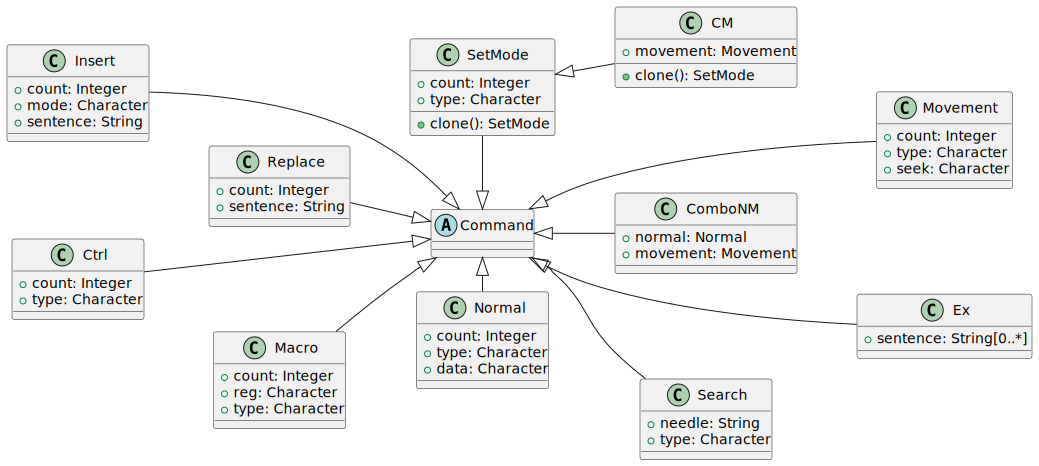
\includegraphics[width=\textwidth]{uml1}
Figure 1. Command Heirarchy updated to include \texttt{CM}, 
\texttt{Search}, and any renamed fields. 
\\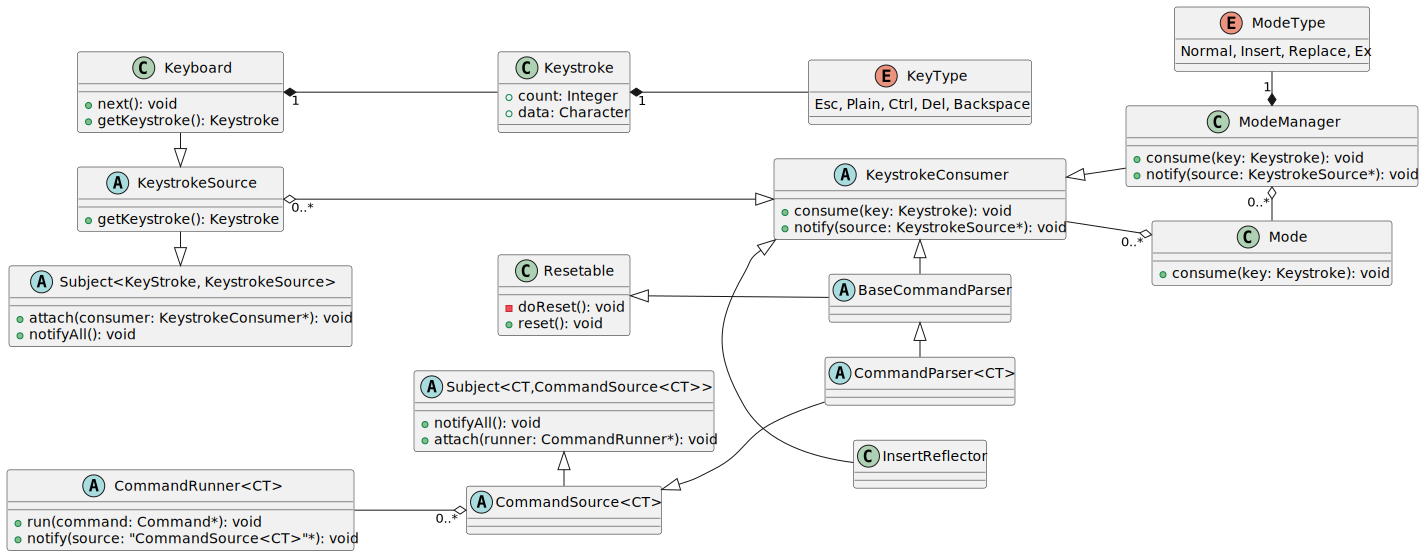
\includegraphics[width=\textwidth]{uml2}
Figure 2. Subjects and objects for \texttt{KeyStroke}s and 
\texttt{Command}, including their templates (see \textbf{Observer Patter})
\\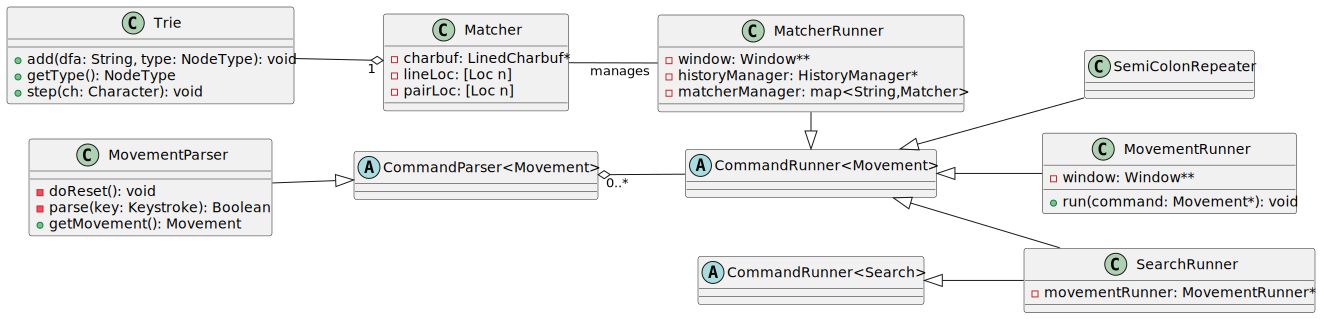
\includegraphics[width=\textwidth]{uml4}
\\\includegraphics[width=\textwidth]{uml3}
\\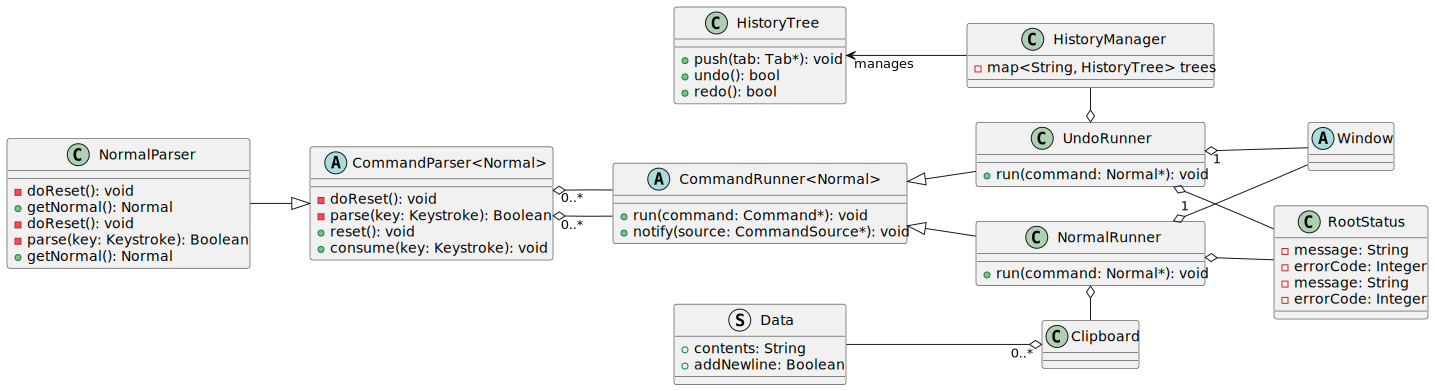
\includegraphics[width=\textwidth]{uml5}
\\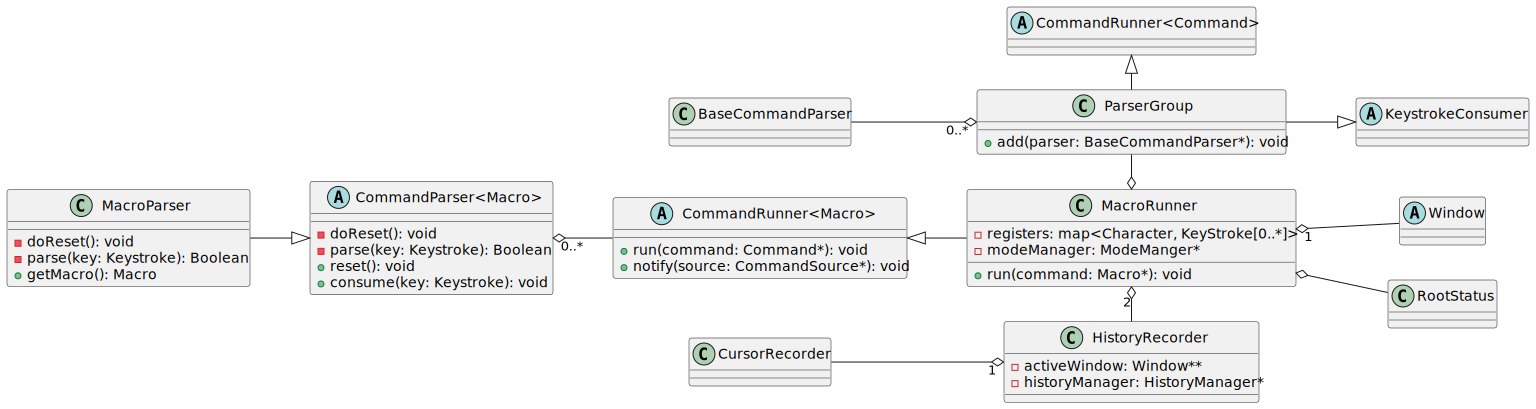
\includegraphics[width=\textwidth]{uml6}
Figure 3. Some selected parsers, runners, and model classes 
for implementing \texttt{ComboNM}, \texttt{Movement}, 
\texttt{Normal}, and \texttt{Macro} commands, in order from top to bottom. 
\\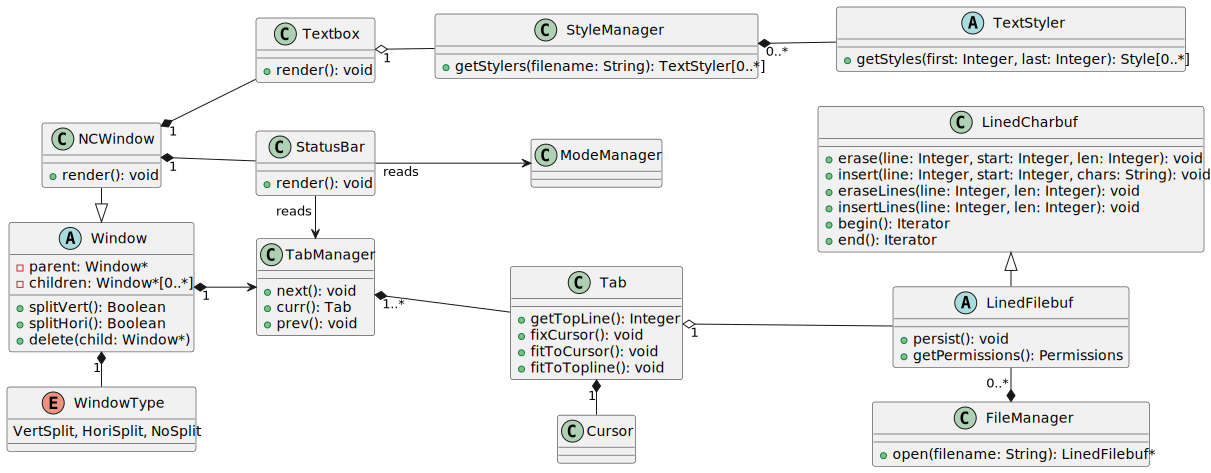
\includegraphics[width=\textwidth]{uml7}
Figure 4. Above: view classes \texttt{NCWindow}, \texttt{Textbox}, \texttt{StatusBar}, 
as well as model classes \texttt{Tab}, \texttt{LinedFilebuf}, 
their managers, and \texttt{Window}. 
Below: separated interfaces of above classes 
in order to adhere to interface segregation principle. 
\\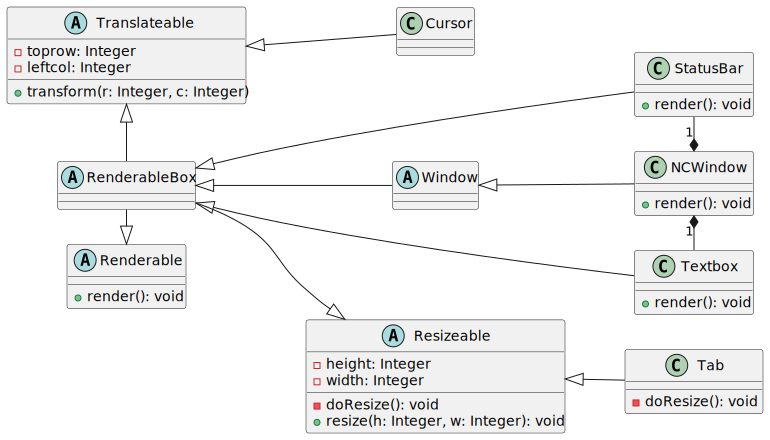
\includegraphics[width=250pt]{uml8}
\\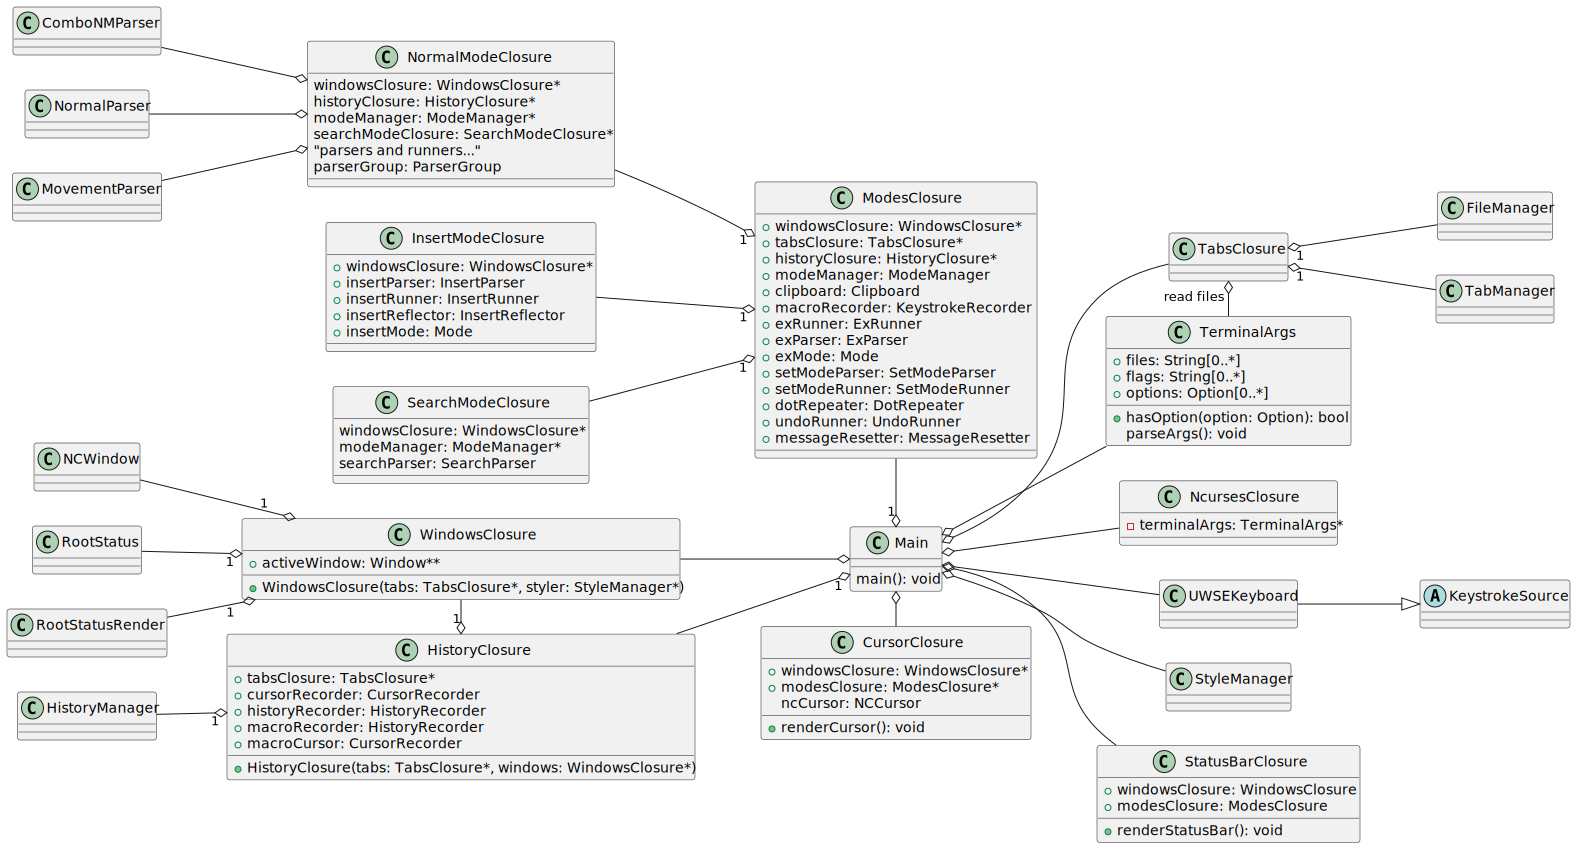
\includegraphics[width=\textwidth]{uml9}
Figure 5. Classes used in \texttt{Main} to RAII and initialize and attach 
all parsers and runners. 

\end{document}
